\documentclass[11pt]{article}
\usepackage[bordered]{uni-style}
\usepackage{wrapfig}
\usepackage{capt-of}
\usepackage{multicol}
\usepackage{threeparttable} % Required for the threeparttable environment
\usepackage{booktabs} % Required for the \toprule, \midrule, and \bottomrule commands
\usepackage{multirow} % Required for the \multirow command
\usepackage{tikz}
\usetikzlibrary{automata, arrows.meta, positioning}
\title{ساختار کامپیوتر و میکروپروسسور}
\prof{دکتر باقری شورکی}
\subtitle{طراحی یک میکروپروفسور}
\subject{پروژه ترم}
\department{مهندسی برق}
\info{
    \begin{tabular}{rl}
        برنا خدابنده & 400109898\\
    \end{tabular}
}
\date{\today}
\usepackage{xepersian}
\settextfont{Yas}

\begin{document}
\maketitlepage
\maketitlestart

\section{تعریف پروژه}

به دنبال طراحی دستگاهی هستیم که به طور خلاصه، شبیه ساز یک
پردازنده، داخل یک پردازنده، است. چنین دستگاهی وظیفه دارد تا
به صورت \lr{Real-time} \textbf{برنامه نویسی} شود. و همینطور در
اتمام برنامه، برنامه نوشته شده را اجرا نیز کند، بدین صورت که داخل
پردازش خود، باید مراحلی که یک پردازنده طی میکند اعم از
\lr{Fetch, Decode, Execute} را داخل خود شبیه سازی کند، ولی این
کار باید کاملا نرم افزاری باشد یعنی در عمل سخت افزار یک پردازنده را
به صورت نرم افزاری باید شبیه سازی کنیم.

طراحی چنین ماشینی در عمل انجام شدنی است زیرا تمامی مراحل طی شده
اعم از اجرا کد و نوشته شدن کد، یک مسئله تشخیص پذیر است و میتوان آن را
به صورت یک \lr{Finite State Machine} پیاده سازی کرد.

\subsection{توصیف عملکرد}

\textbf{فرایند برنامه نویسی : }
این فرایند در واقع فقط نیاز دارد تا در آدرس های حافظه دلخواه، داده دلخواه توسط کاربر وارد
و ذخیره شود، این اطلاعات میتوانند هم به صورت \lr{OPCODE} و هم به صورت \lr{OPERAND} باشند،
برای پردازنده ما تفاوتی وجود ندارد.

روند برنامه نوشتن به شکل زیر است.

\begin{enumerate}
	\item دکمه \lr{ORG} زده میشود.
	\item یک عدد 2 رقمی به عنوان آدرس وارد میشود.
	\item دکمه \lr{EXE} برای تایید زده میشود.
	\item در این آدرس عددی 2 رقمی به عنوان \lr{OPCODE} یا \lr{OPERAND} قرار داده میشود.
	\item دکمه \lr{EXE} برای تایید زده میشود.
	\item با کلید های + یا - و یا دوباره با ORG به آدرس جدید میرویم.
\end{enumerate}

همچنین بعضی از کلید ها مانند \texttt{F1-F8} را تعبیه کردیم که کار های خاص را انجام میدهد،
برای مثال \texttt{F1} هر زمانی زده شود محتوای Accumilator را نمایش داده و \texttt{F2} برای ما state در
حال حاضر را نشان میدهد.

\vfil
\begin{figure}[h]
	\centering
	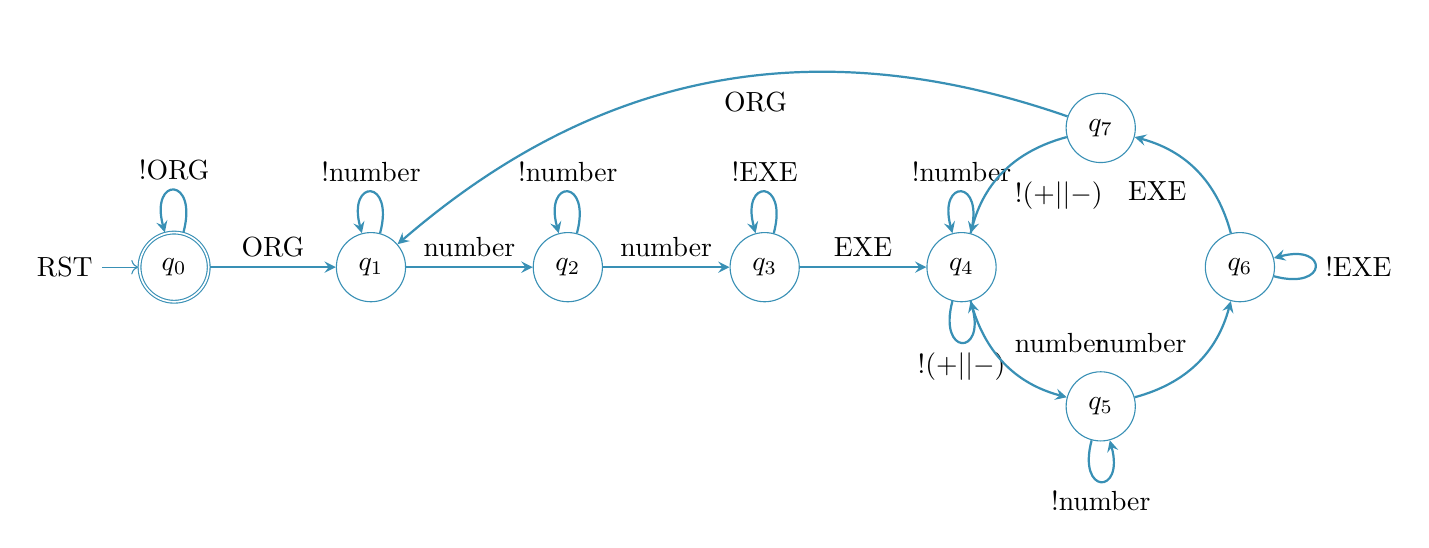
\begin{tikzpicture} [draw=cyan!70!black,
			node distance = 2.5cm,
			on grid,
			auto,
			every loop/.style={stealth-},
		]

		% State q0 
		\node (q0) [state,
			initial,
			accepting,
			initial text = {RST}] {$q_0$};
		% States    
		\node (q1) [state,
			right = of q0] {$q_1$};
		\node (q2) [state,
			right = of q1] {$q_2$};
		\node (q3) [state,
			right = of q2] {$q_3$};
		\node (q4) [state,
			right = of q3] {$q_4$};
		\node (q7) [state,
			above right = of q4] {$q_7$};
		\node (q5) [state,
			below right = of q4] {$q_5$};
		\node (q6) [state,
			below right = of q7] {$q_6$};
		% Arrows
		\path [-stealth, thick]
		% (q0) edge[bend left] node {$a$}   (q1)
		% (q1) edge[bend left] node {$b$}   (q0)
		% (q0) edge [loop above]  node {b}()
		% (q1) edge [loop above]  node {b}();
		(q0) edge node {ORG} (q1)
		(q0) edge[loop above] node {!ORG} (q0)
		(q1) edge [loop above] node {!number} (q1)
		(q1) edge node {number} (q2)
		(q2) edge [loop above] node {!number} (q2)
		(q2) edge node {number} (q3)
		(q3) edge [loop above] node {!EXE} (q3)
		(q3) edge node {EXE} (q4)
		(q4) edge [loop above] node {!number} (q4)
		(q4) edge [loop below] node {$!(+||-)$} (q4)
		(q4) edge[bend right] node {number} (q5)
		(q5) edge [loop below] node {!number} (q5)
		(q5) edge[bend right] node {number} (q6)
		(q6) edge [loop right] node {!EXE} (q6)
		(q6) edge[bend right] node {EXE} (q7)
		(q7) edge [bend right] node {$!(+||-)$} (q4)
		(q7) edge [bend right] node {ORG} (q1)
		;
	\end{tikzpicture}
	\caption{برنامه نویسی}
\end{figure}

\clearpage

\begin{figure}[h]
	\centering
	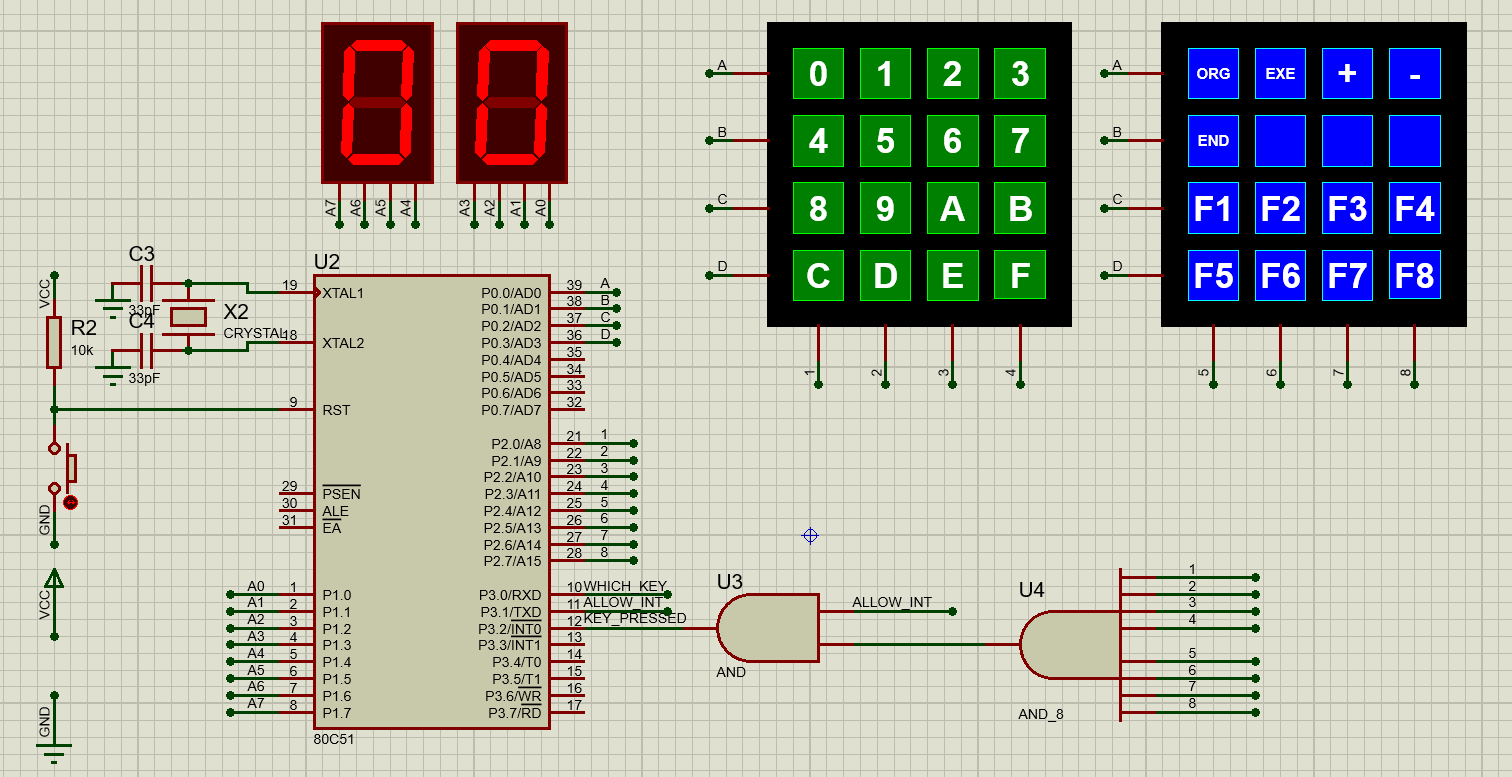
\includegraphics[width=0.9\linewidth]{result/schematics.png}
	\caption{شماتیک طرح}
\end{figure}

\section{چالش ها}

برای حالت های مختلف، رجیستر ها را به شکل زیر توصیف میکنیم تا مشکلات کمتری را بر بخوریم.

با تعریف یک رجیستر جداگانه برای PC مشکلاتی که ممکن بود برای  پیاده سازی JMP
داشته باشیم از بین می رود.

فقط برای STACK نیاز داشتیم تا مکانی از حافظه را اختصاص دهیم و یک SPTR تعریف کنیم،
ولی برا این منظور نیاز داشتیم رجیستر R0 که دسترسی به آن به صورت آدرس را داریم را نیز
از بین ببریم، پس میکروپروفسور ما از قابلیت ها رفرنس آدرس دیگر بهره مند
نمیبود، میتوانستیم با استفاده از برنامه های پیچیده تر و توصیف بخشی از
حافظه به عنوان STACK این عمل را انجام دهیم، ولی برای سادگی در این پیاده سازی فقط یک
رجیستر را به عنوان STACK در نظر گرفته ایم.

کد کامل برای این ماشین درج شده است.
\begin{table}[ht]
	\centering
	\begin{threeparttable}
		\caption{آدرس‌ها}
		\label{tbl:addresses}

		\begin{tabular}{lcr}
			\toprule
			\multicolumn{1}{c}{\textbf{حالت کدنویسی}} & \multicolumn{1}{c}{\textbf{آدرس‌ها}} & \multicolumn{1}{c}{\textbf{آدرس‌ها}} \\
			\midrule
			\multirow{4}{*}{\textbf{در حالت کدنویسی}} &
			\lr{R0}                                   & وضعیت FSM                                                                 \\
			                                          & \lr{R1}                             & ورودی                               \\
			                                          & \lr{R2}                             & داده ورودی                          \\
			                                          & \lr{R3}                             & آدرس ورودی                          \\
			\midrule
			\multirow{4}{*}{\textbf{در حالت اجرا}}    &
			\lr{R6}                                   & آدرس شروع                                                                 \\
			                                          & \lr{R1}                             & PC (شمارنده برنامه)                 \\
			                                          & \lr{R3}                             & پشته                                \\
			                                          & \lr{R4}                             & IR (ثبت دستور)                      \\
			\bottomrule
		\end{tabular}

		\begin{tablenotes}
			\item[] منبع: ایجاد توسط نویسنده.
		\end{tablenotes}

	\end{threeparttable}
\end{table}

حالت کد نویسی توصیف شده، حالت اجرا نیز قابل ساخت است، بدین صورت که کافسیست fetch, decode, Execute را
شبیه سازی کنیم، در کد درج شده هست، ولی برای مثال برای پیاده سازی یک اینستراکشن خاص:

\begin{latin}
	\begin{verbatim}
		ADD_R2_MNEMONIC: CJNE R4, #02AH, ADD_R5_MNEMONIC
        	ADD A, R2
    	RET
	\end{verbatim}
\end{latin}

\clearpage

\section{تست کاربر}

با استفاده از کد زیر، کار گفته شده را انجام میدهیم.
\begin{latin}
	\begin{verbatim}
		MOV R2, #n   ; Set n to the desired value
		MOV R0, #m   ; Set R1 to the starting address m
		MOV R5, #1   ; Initialize R2 to hold the current number
		LOOP:
		MOV A, R5
		MOV @R0, A   ; Write the current number to the memory location pointed by R1
		
		INC R0       ; Increment the memory address
		INC R5       ; Increment the current number
		
		; Decrement n and repeat the loop if not zero
		DEC R2
		MOV A, R2    
		JNZ LOOP
	\end{verbatim}
\end{latin}

حال فقط کافیست تا که کد بالا را روی میکروپروفسور خود قرار دهیم. کد معادل به صورت عددی به شکل زیر است.

\begin{latin}
	\begin{verbatim}
		64: 7A (MOV R2, #data)
65: n
66: 78 (MOV R0, #data)
67: m
68: 7D (MOV A, #data)
69: 01
6A: ED (MOV A, R5)
6B: F6 (MOV @R0, A)
6C: 08 (INC R0)
6D: 0D (INC R5)
6E: 1A (DEC R2)
6F: EA (MOV A, R2)
70: 70 (JNZ reladdr)
71: 6A
	\end{verbatim}
\end{latin}

حال بعد از وارد کردن این کد داخل میکروپروفسور به طور توصیف شده و اجرا، میبینیم که
این اتفاق انجام میشود.

بدین صورت که کد را قرار میدهیم، END را میزنیم، و سپس بعد از RESET با استفاده از
ORG و یا +, - به آدرس مد نظر میرویم و میبینیم که داده مورد نظر در آنجا ذخیره شده استو.
\vfil

\begin{conclusion}
	در آخر ما موفق به ساخت چنین دستگاهی شدیم، بدین صورت که حال میکروپروفسور ای
	داریم که هر کد اسمبلی ای که به آن دهیم را میتواند مانند یک پروسسور واقعی ( با یک سری محدودیت بیشتر )
	به صورت \lr{Real-time} اجرا کند و برنامه ریزی شود.

	چالش های زیادی در این پیاده سازی داشتیم، اعم از
	کد کردن ورودی از صفحه کلید به اپراتور های داخل میکروپروفسور،
	ذخیره درست اطلاعات، پیاده سازی برنامه ریزی میکروپروفسور به صورت نرم افزاری و با صفحه کلید، توصیف
	برنامه نویسی به صورت یک FSM, پیاده سازی و آپدیت مناسب این FSM،
	و در نهایت چالش کمتری ولی چالش برای شبیه سازی سیکل اجرای برنامه در داخل پروسسور.

	این قسمت آخر در واقع محدودیت اصلی ما را ایجاد کرده زیرا بعضی از رجیستر ها
	صرف رجیستر های داخلی این پروسسور نرم افزاری میشوند، همچنین این پروسسور نرم افزاری
	دیگر قابلیت تعامل با دنیای خارجی به صورت I/O را ندارد.

	در نهایت با استفاده از حداقل رجیستر های پروسسور، و پیاده سازی مناسب FSM توانستیم
	سیکل های برنامه نویسی و سیکل اجرا را به صورت نرم افزاری شبیه سازی کنیم و یک
	میکروپروفسور بسازیم.
\end{conclusion}

\clearpage

\section{نتایج تست}

تست شده با $m=A0$, $n=10$

عکس زیر داده های خانه $A0$ و $B0$ است.
\begin{figure}[h]
	\centering
	\includegraphics*[width=0.45\linewidth]{result/firstnum.png}
	\includegraphics*[width=0.45\linewidth]{result/lastnum.png}
	\caption{اعداد اول و آخر ذخیره شده}
\end{figure}

\subsubsection{تست های دیگر}

کد برای محاسبه $m+n$:
\begin{latin}
	\begin{verbatim}
		MOV A, #02H : 74, m
ADD A, #03H : 24, n
NOP         : 00
	\end{verbatim}
\end{latin}

\begin{figure}[h]
	\centering
	\includegraphics*[width=0.45\linewidth]{result/calculation 2+3.png}
	\caption{نتیجه برای محاسبه 2+3}
\end{figure}

محاسبه برای $m*n$
\begin{figure}[h]
	\centering
	\begin{minipage}[r]{0.5\linewidth}
		\centering
		\includegraphics*[width=\linewidth]{result/calculation 2x3.png}
	\end{minipage}
	\begin{minipage}[l]{0.4\linewidth}
		\begin{latin}
			\begin{verbatim}
				MOV R4, n
				MOV R7, m
				MOV A, #00H ; result register
				LOOP:
				MOV A, R5
				ADD A, R4
				MOV R5, A
				DEC R7
				MOV A, R3
				JNZ LOOP
			\end{verbatim}
		\end{latin}
	\end{minipage}
	\caption{نتیجه برای محاسبه 2*3}
\end{figure}
\end{document}